\newpage
\section{Experiment - 1: I-V characteristics of MOS transistors}
\subsection{NMOS}
\begin{figure}[H]
	\centering
	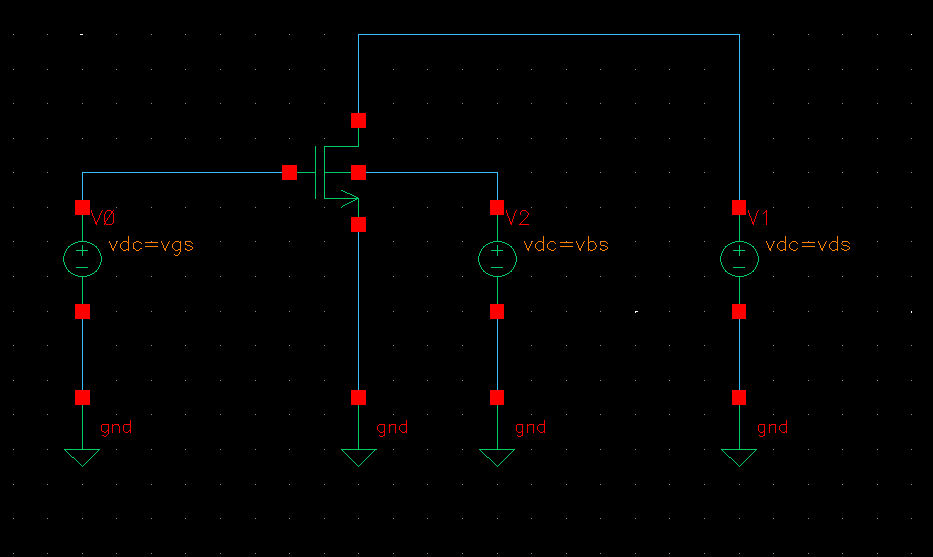
\includegraphics[width = 0.6\linewidth]{sections/pic/EX1_NMOS.png}
	\caption{Test setup for the NMOS\_VTG transistor.}
	\label{f_ex1NMOS-schematic}
\end{figure}

\itemmini{Simulate curves $I_D$ vs $V_{DS}$ @ $V_{GS} = 1V$, and sweeping variable $V_{DS} = [0, 1.5](V)$ step $10mV$.}

\begin{figure}[H]
	\centering
	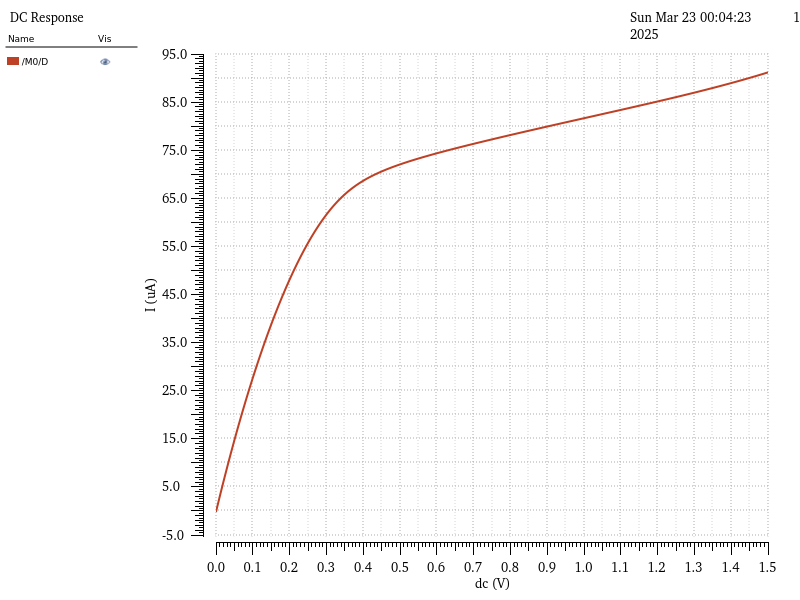
\includegraphics[width=0.6\linewidth]{sections/pic/EX1_NMOS_Id&Vds(Vgs1).png}
	\caption{$I_D$ vs $V_{DS}$ @ $V_{GS} = 1V$, and sweeping variable $V_{DS} = [0, 1.5](V)$ step $10mV$.}
	\label{f_EX1_NMOS_Id&Vds(Vgs1)}
\end{figure}

\begin{discussion}
	\item With \( V_{GS} = 1 \), a conductive channel is formed. Increasing \( V_{DS} \) will increase \( I_{DS} \). For small \( V_{DS} \), \( I_{DS} \) increases linearly, and this region is called the triode region.
	\item When \( V_{DS} \) increases further, entering the saturation region, \( I_{DS} \) does not remain constant as in the ideal model. Instead, it increases slightly due to the channel length modulation effect, which reduces resistance and increases the drain current \( I_{DS} \).
\end{discussion}

\itemmini{Simulate curves $I_D$ vs $V_{GS}$ @ $V_{DS} = 1.5V$, and sweeping variable $V_{GS} = [0, 1.5](V)$ step $10mV$.} 

\begin{figure}[H]
	\centering
	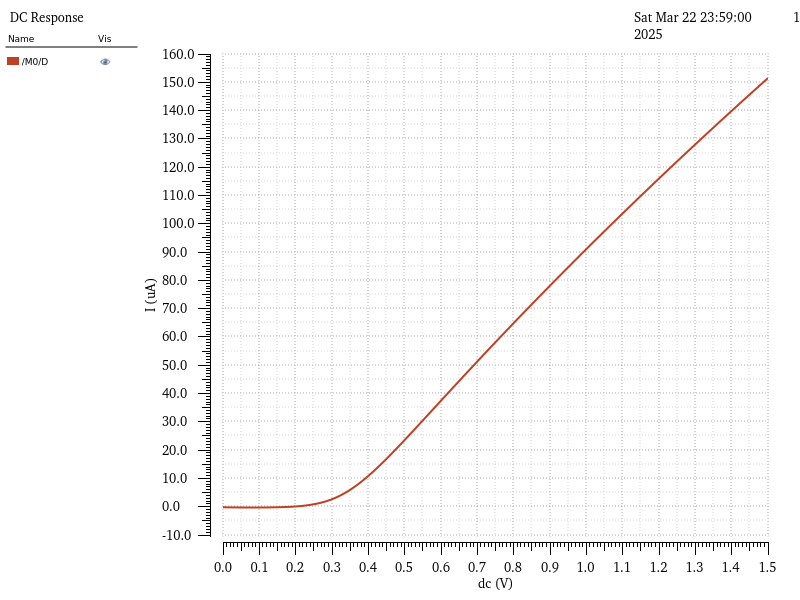
\includegraphics[width=0.6\linewidth]{sections/pic/EX1_NMOS_Id&Vgs(Vds15).png}
	\caption{$I_D$ vs $V_{GS}$ @ $V_{DS} = 1.5V$, and sweeping variable $V_{GS} = [0, 1.5](V)$ step $10mV$.}
	\label{f_EX1_NMOS_Id&Vgs(Vds15)}
\end{figure}

\begin{discussion}
	\item Initially, when \( V_{GS} < V_{TH} \), the NMOS does not form a conductive channel, and the drain-to-source current \( I_{DS} \) is always zero. However, when \( V_{GS} > V_{TH} \), the conductive channel forms, allowing current to flow from the drain to the source. At this point, we can say that the NMOS enters the conduction region.
\end{discussion}

\subsection{PMOS}
\begin{figure}[H]
	\centering
	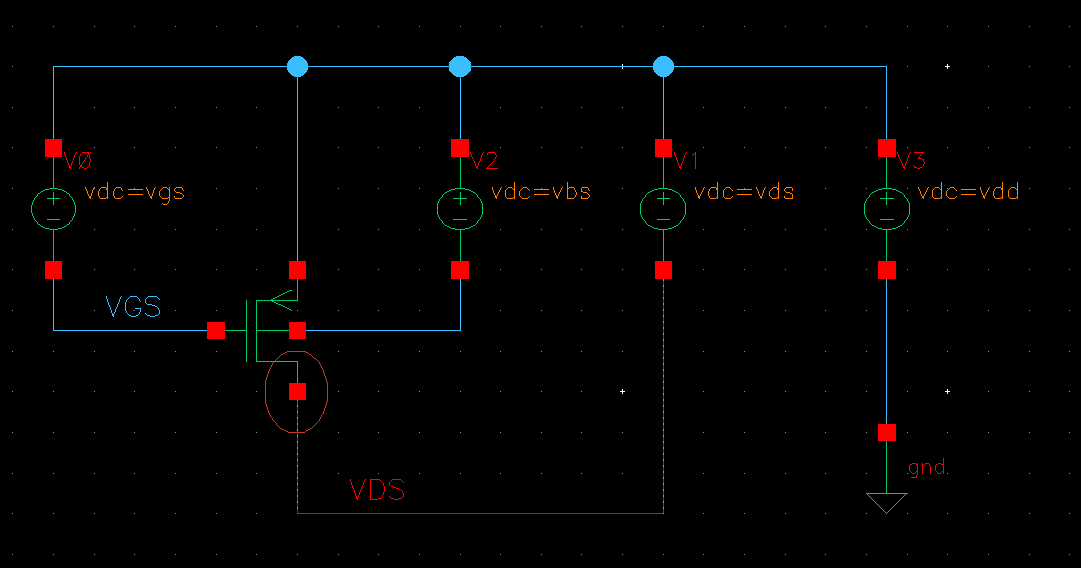
\includegraphics[width = 0.6\linewidth]{sections/pic/EX1_PMOS.png}
	\caption{Test setup for the PMOS\_VTG transistor.}
	\label{f_ex1PMOS-schematic}
\end{figure}

\itemmini{Simulate curves $I_D$ vs $V_{DS}$ @ $V_{SG} = 1V$, and sweeping variable $V_{SD} = [0, 1.5](V)$ step $10mV$.}

\begin{figure}[H]
	\centering
	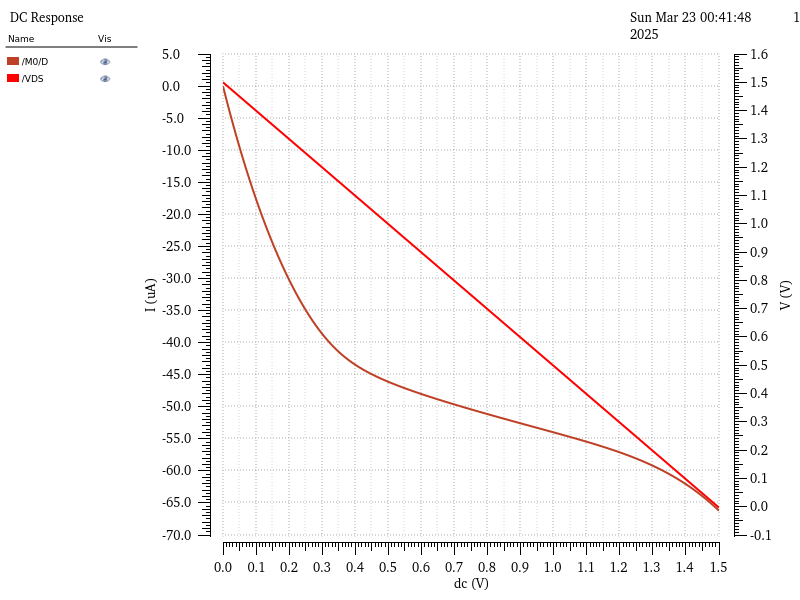
\includegraphics[width=0.6\linewidth]{sections/pic/EX1_PMOS_Id&Vds(Vgs1).png}
	\caption{$I_D$ vs $V_{DS}$ @ $V_{SG} = 1V$, and sweeping variable $V_{SD} = [0, 1.5](V)$ step $10mV$.}
	\label{f_EX1_PMOS_Id&Vds(Vgs1)}
\end{figure}

\itemmini{Simulate curves $I_D$ vs $V_{GS}$ @ $V_{SD} = 1.5V$, and sweeping variable $V_{SG} = [0, 1.5](V)$ step $10mV$.}

\begin{figure}[H]
	\centering
	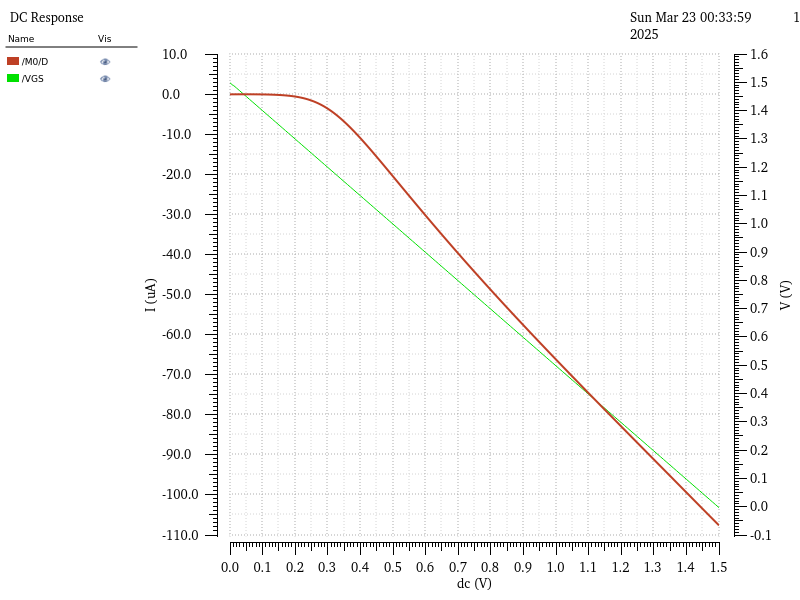
\includegraphics[width=0.6\linewidth]{sections/pic/EX1_PMOS_Id&Vgs(Vds15).png}
	\caption{$I_D$ vs $V_{GS}$ @ $V_{SD} = 1.5V$, and sweeping variable $V_{SG} = [0, 1.5](V)$ step $10mV$.}
	\label{f_EX1_PMOS_Id&Vgs(Vds15)}
\end{figure}

\begin{question}
	\item Based on the $I_D$ vs $V_{GS}$ characteristics, please estimate the threshold voltage $V_{GS}$ of the NMOS transistor. 
	
	\begin{answer}
		In Figure~\ref{f_EX1_NMOS_Id&Vgs(Vds15)}, when \( V_{GS} = 0.28\,\mathrm{V} \), the drain current \( I_{DS} \) begins to increase (deviating from zero). Therefore, the threshold voltage is estimated as \( V_{Th} = 0.28\,\mathrm{V} \) by our group based on the graph.
	\end{answer}
	
	\item Additionally, by analyzing the $I_{D}$ vs $V_{DS}$ characteristics, determine the conduction region of the NMOS transistor when $V_{GS}$ exceeds $V_{Th}$. Specify whether the device operates in the linear (triode) region or the saturation region and provide an explanation.
	
	\begin{answer}
		It is easy to recognize the conduction region of an NMOS transistor when examining the $I_{D}$ versus $V_{GS}$ characteristics. When $V_{GS}$ exceeds $V_{Th}$ (which our group calculated in Question 1), the drain current $I_{DS}$ begins to increase.
		
		$\Rightarrow$ This is the conduction region.
		 		
		The more challenging task is distinguishing between the linear (ohmic) region and the saturation region within the conduction region.
		
		\begin{itemize}[label=-]
			\item The conditions for NMOS operation in the saturation region are:
			\[ 
			V_{GS} > V_{Th} \quad \text{and} \quad V_{DS} \geq V_{GS} - V_{Th}
			\]
			
			\item In the $I_{D}$-$V_{GS}$ characteristics, these conditions are satisfied.
		\end{itemize}
		
		$\Rightarrow$ This represents the saturation region within the conduction region.
	\end{answer}
	
	\item Based on Figure \ref{f_EX1_NMOS_Id&Vds(Vgs1)}, qualitatively determine the operating regions of the NMOS transistor.
	
	\begin{answer}
		\begin{itemize}[label=-]
			\item We see that at $V_{DS} = 0.5V$ the V-I characteristics changing from Triode Region into saturation region.
			
			\item We can calculate the $V_{Th} = V_{GS} - V_{DS} = 0.5(V)$
			
			\item With this result, we can draw operating region table:
			
			\begin{tabular}{|p{0.4\linewidth} | p{0.4\linewidth} |}
				\hline
				Requirements & Operation \\
				\hline
				$V_{GS} < V_{Th} = 0.5$ & Cut off \\
				\hline
				$V_{DS} < V_{GS} - V_{Th} = 0.5$ & Linear \\
				\hline
				$V_{DS} > V_{GS} - V_{Th} = 0.5$ & Saturation\\
				\hline
			\end{tabular} 
		\end{itemize}
	\end{answer}
	
	\item When the NMOS transistor is biased in the saturation region, does the drain current remain constant? Provide a theoretical explanation.
	
	\begin{answer}
		Based on long-channel, ideal, first-order, or Shockley model:
		
		\begin{itemize}[label=-]
			\item At saturation region, based on equation, the drain current remain constant at:
			
			\[ I_{DS} = \dfrac{1}{2} \mu C_{ox} \dfrac{W}{L} (V_{GS} - V_{T})^{2}\]
			
			\item Moreover, with the ideal model we assume that channel-length modulation does not exit, the length of NMOS do not decreasing when $V_{DS}$ increases.
			
		\end{itemize}
		
		$\Rightarrow$ The current $I_{DS}$ do remain in ideal model.
		
		Based on non-ideal model:
		
		\begin{itemize}[label=-]
			\item In non-ideal model, the length of NMOS will decrease when $I_{DS}$ increases leading to the p-n junction between the drain and body forms a depletion region.
			
			\item When the length of the NMOS decreases, it leads to the slightly raising of the current $I_{DS}$ (because resistor value decrease).
			
			\item We have the current equation of $I_{DS}$ in ideal model:
			\begin{align}
				I_{DS} = \dfrac{\beta}{2} V_{GS}^{2} \left(1 + \dfrac{V_{GS}}{V_{A}}\right) \label{eq_EX1_NMOS_ques3}
			\end{align}
		\end{itemize}
		
		$\Rightarrow$ The current $I_{DS}$ do not remain in non-ideal model.
	\end{answer}
	
	\item Propose methods to reduce the slope of the drain current when the NMOS operates in the saturation region. 
	
	\begin{answer}
		\begin{itemize}[label=-]
			\item We increase the length of the NMOS, which reduces the effect of changes in the depletion region between the drain and body on the current, $I_{DS}$.
			\item Based on equation the slope of the current is inverse ratio with L, so L increasing then the current will decrease (Equation \ref{eq_EX1_NMOS_ques3}).
		\end{itemize}
	\end{answer}
\end{question}